\documentclass{article}
\usepackage{amsmath, amssymb, amsthm}
\usepackage{tikz}
\usetikzlibrary{shapes.geometric, arrows.meta, positioning}

\theoremstyle{plain}
\newtheorem{theorem}{Theorem}[section]
\newtheorem{lemma}[theorem]{Lemma}
\newtheorem{proposition}[theorem]{Proposition}
\newtheorem{corollary}[theorem]{Corollary}
\newtheorem{definition}[theorem]{Definition}
\newtheorem*{remark}{Remark}
\theoremstyle{remark}

\begin{document}

\title{Issue XXIV: Locally Cartesian Closed Categories}
\author{Namdak Tonpa}
\date{May 5, 2025}

\maketitle

\begin{abstract}
We introduce locally cartesian closed categories (LCCCs), a class of categories where each slice category is cartesian closed. Definitions of categories, slice categories, and cartesian closed categories are provided, followed by the formal definition of LCCCs. We discuss their significance in categorical logic and dependent type theory, including a theorem on their correspondence to type theories with dependent products
\end{abstract}

\ifincludeTOC
  \tableofcontents
\fi

\section{Locally Cartesian Closed Categories}

\subsection{Definitions}

Locally cartesian closed categories (LCCCs) are categories where each slice category $\mathcal{C}/x$ is cartesian closed, meaning it has products, exponentials, and a terminal object. LCCCs are fundamental in categorical logic, providing models for dependent type theories with dependent products. This article defines the necessary structures, presents key properties, and highlights their role in type theory, with references from the nLab.

\begin{definition}[Cartesian Closed Category]
A \emph{cartesian closed category} (CCC) is a category $\mathcal{C}$ equipped with:
\begin{itemize}
    \item A \emph{terminal object} $1 \in \mathrm{ob}(\mathcal{C})$, such that for every $x \in \mathrm{ob}(\mathcal{C})$, there exists a unique morphism $!_x : x \to 1$.
    \item For each pair $A, B \in \mathrm{ob}(\mathcal{C})$, a \emph{product} $A \times B \in \mathrm{ob}(\mathcal{C})$ with projections $p_1 : A \times B \to A$, $p_2 : A \times B \to B$, and a universal property: for any $X \in \mathrm{ob}(\mathcal{C})$ with morphisms $f : X \to A$, $g : X \to B$, there exists a unique $\langle f, g \rangle : X \to A \times B$ such that $p_1 \circ \langle f, g \rangle = f$ and $p_2 \circ \langle f, g \rangle = g$.
    \[
    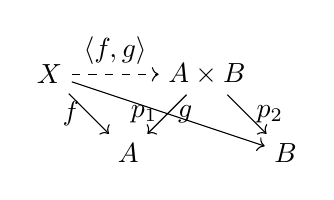
\begin{tikzpicture}
        \node (X) at (0,1) {$X$};
        \node (AB) at (2,1) {$A \times B$};
        \node (A) at (1,0) {$A$};
        \node (B) at (3,0) {$B$};
        \draw[->, dashed] (X) to node[above] {$\langle f, g \rangle$} (AB);
        \draw[->] (X) to node[left] {$f$} (A);
        \draw[->] (X) to node[right] {$g$} (B);
        \draw[->] (AB) to node[left] {$p_1$} (A);
        \draw[->] (AB) to node[right] {$p_2$} (B);
    \end{tikzpicture}
    \]
    \item For each pair $A, B \in \mathrm{ob}(\mathcal{C})$, an \emph{exponential object} $B^A \in \mathrm{ob}(\mathcal{C})$ with an evaluation morphism $\mathrm{ev} : B^A \times A \to B$, and a universal property: for any $X \in \mathrm{ob}(\mathcal{C})$ with $f : X \times A \to B$, there exists a unique $\lambda f : X \to B^A$ such that $\mathrm{ev} \circ (\lambda f \times \mathrm{id}_A) = f$.
    \[
    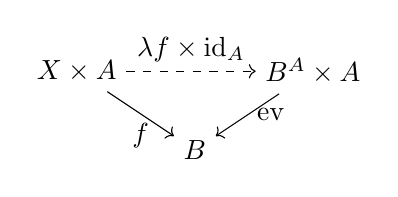
\begin{tikzpicture}
        \node (XA) at (0,1) {$X \times A$};
        \node (BAxA) at (3,1) {$B^A \times A$};
        \node (B) at (1.5,0) {$B$};
        \draw[->, dashed] (XA) to node[above] {$\lambda f \times \mathrm{id}_A$} (BAxA);
        \draw[->] (XA) to node[below] {$f$} (B);
        \draw[->] (BAxA) to node[right] {$\mathrm{ev}$} (B);
    \end{tikzpicture}
    \]
\end{itemize}
\end{definition}

\begin{remark}
A CCC has finite products (via the terminal object and binary products) and internal homs (via exponentials), making it a model for simply typed lambda calculus.
\end{remark}

\begin{definition}[Locally Cartesian Closed Category]
A category $\mathcal{C}$ is \emph{locally cartesian closed} if, for every object $x \in \mathrm{ob}(\mathcal{C})$, the slice category $\mathcal{C}/x$ is cartesian closed, i.e., $\mathcal{C}/x$ has a terminal object, binary products, and exponential objects.
\end{definition}

\subsection{Theorems}

\begin{theorem}[LCCCs and Dependent Type Theory]
\label{thm:lccc-type-theory}
(Seely, \cite{Seely87}) A locally cartesian closed category $\mathcal{C}$ provides a categorical model for a dependent type theory with dependent products. Conversely, any dependent type theory with dependent sums and products can be interpreted in an LCCC.
\end{theorem}

\begin{proof}[Sketch]
In an LCCC $\mathcal{C}$, the slice category $\mathcal{C}/x$ models the context of types over a base type $x$. The terminal object in $\mathcal{C}/x$ corresponds to the trivial type, products in $\mathcal{C}/x$ correspond to dependent pairs, and exponentials model dependent function types. The pullback functor along morphisms $f : y \to x$ in $\mathcal{C}$ corresponds to substitution in type theory. The universal properties of products and exponentials in each $\mathcal{C}/x$ ensure the rules of dependent products are satisfied. Conversely, a type theory with dependent sums and products constructs an LCCC via its syntactic category, where contexts are objects and terms are morphisms.
\end{proof}


\subsection{Examples}

\begin{enumerate}
    \item The category $\mathbf{Set}$ of sets is locally cartesian closed. For any set $X$, the slice category $\mathbf{Set}/X$ is equivalent to the category of $X$-indexed families of sets, which has products, exponentials, and a terminal object (the identity family).
    \item The category $\mathbf{Top}$ of topological spaces is not locally cartesian closed, as not all slice categories $\mathbf{Top}/X$ are cartesian closed (e.g., exponentials may not exist for arbitrary spaces).
    \item The category of presheaves $\mathbf{Set}^{\mathcal{C}^{\mathrm{op}}}$ on a small category $\mathcal{C}$ is locally cartesian closed, as each slice $\mathbf{Set}^{\mathcal{C}^{\mathrm{op}}}/F$ is equivalent to a presheaf category over a comma category, which is cartesian closed.
\end{enumerate}

\subsection{Conclusion}

Locally cartesian closed categories bridge category theory and dependent type theory, providing a semantic framework for modeling complex type systems. Their slice categories’ cartesian closed structure supports dependent products, making them a powerful tool in categorical logic. Theorem \ref{thm:lccc-type-theory} underscores their significance, and examples like $\mathbf{Set}$ illustrate their applicability.

\begin{thebibliography}{9}

\bibitem{Awodey10} S. Awodey, \emph{Category Theory}, Oxford Logic Guides, Vol. 49, Oxford University Press, 2010.
\bibitem{Johnstone02} P. T. Johnstone, \emph{Sketches of an Elephant: A Topos Theory Compendium}, Oxford Logic Guides, Vol. 43–44, Oxford University Press, 2002.
\bibitem{Seely87} R. A. G. Seely, \emph{Locally cartesian closed categories and type theory}, Mathematical Proceedings of the Cambridge Philosophical Society, Vol. 95, No. 1, 1987, pp. 33--48.

\end{thebibliography}


\end{document}
